\documentclass[a4paper]{report}
\usepackage[T2A,T1]{fontenc}
\usepackage[utf8]{inputenc}
\usepackage{blindtext}
\usepackage[russian]{babel}
\usepackage{mwe}
\usepackage{graphbox}
\usepackage[document]{ragged2e}
\usepackage[margin=0.8in]{geometry}
\usepackage{longtable}
\usepackage{minted}

\graphicspath{{./images/}}

\begin{document}
	Сысойкин Егор, ИУ5-54Б
	\section*{Условие}
	Вариант запросов - Г.
	Вариант ПО - 20.
	\begin{enumerate}
    	\item «Поставщик» и «Деталь» связаны соотношением один-ко-многим. Выведите список всех поставщиков, у которых название начинается с буквы «А», и список деталей, которые они поставляют. \\
    	\item «Поставщик» и «Деталь» связаны соотношением один-ко-многим. Выведите список поставщиков с максимальной стоимостью деталей для каждого поставщика, отсортированный по максимальной стоимости. \\
    	\item «Поставщик» и «Деталь» связаны соотношением многие-ко-многим. Выведите список всех связанных деталей и поставщиков, отсортированный по поставщикам, сортировка по деталям произвольная. \\ 
	\end{enumerate}

	\section*{Исходный код программы}

\begin{minted}[linenos]{python}
#!/usr/bin/env python

from operator import itemgetter

class Detail:
	"""Деталь"""
	def __init__(self, id, name, price, supplier_id):
		self.id = id
		self.name = name
		self.price = price
		self.supplier_id = supplier_id

class Supplier:
	"""Поставщик"""
	def __init__(self, id, name):
		self.id = id
		self.name = name

class DetailSupplier:
	"""Деталь к поставщику, для реалиации многие-ко-многим"""
	def __init__(self, detail_id, supplier_id):
		self.detail_id = detail_id
		self.supplier_id = supplier_id


if __name__ == "__main__":
	suppliers = [
		Supplier(0, "ООО ПОСТАВЩИК"),
		Supplier(1, "ААО МЕТАЛЛСТРОЙ"),
		Supplier(2, "МедСклад"),
		Supplier(3, "Акладстрой"),
		Supplier(4, "Трубзавод"),
		Supplier(5, "РусБытХим"),
	]

	details = [
		Detail(0, "Труба пластиковая", 150, 0),		
		Detail(1, "Труба железная", 1500, 1),
		Detail(2, "Труба стекловолоконная", 280, 2),
		Detail(3, "Труба титановая", 164, 3),
		Detail(4, "Ключ", 2080, 3),
		Detail(5, "Часть", 1047, 3),
		Detail(6, "Круг", 1100, 3),
		Detail(7, "Стеклянный кусок", 120, 2),
		Detail(8, "Углеволокно", 130, 2),
		Detail(9, "Кран", 260, 1),
		Detail(10, "Кусочек лего", 320, 4),
		Detail(11, "Доска", 480, 5),
		Detail(12, "Металлическая пластина", 720, 5),
		Detail(13, "Пластиковая пластина", 640, 4),
		Detail(14, "Минеральное стекло", 770, 3),
	]
	
	details_suppliers = [
		DetailSupplier(0, 0),
		DetailSupplier(1, 1),
		DetailSupplier(2, 2),
		DetailSupplier(3, 3),
		DetailSupplier(3, 4),
		DetailSupplier(3, 5),
		DetailSupplier(5, 5),
		DetailSupplier(4, 4),
		DetailSupplier(8, 1),
		DetailSupplier(11, 5),
	]


	 # Соединение данных один-ко-многим 
	one_to_many = [(d.name, d.price, s.name)
        for s in suppliers
        for d in details
        if d.supplier_id==s.id]

    # Соединение данных многие-ко-многим
	many_to_many_temp = [(s.name, ds.supplier_id, ds.detail_id)
		for s in suppliers
		for ds in details_suppliers
		if s.id==ds.supplier_id]
	many_to_many = [(d.name, d.price, supplier_name)
		for supplier_name, supplier_id, detail_id in many_to_many_temp
		for d in details if d.id==detail_id]

	print("Задание А1")
	res_11 = {}
	selected_suppliers = [one_suppl[2] for one_suppl in one_to_many if one_suppl[2].startswith('а') or one_suppl[2].startswith('А')]
	for supplier_name in selected_suppliers:
		details_for_suppl = [(one_detail[0],one_detail[1]) for one_detail in one_to_many if one_detail[2]==supplier_name]
		res_11.update({supplier_name:details_for_suppl})
	print(res_11)
	print()

	print("Задание A2")
	res_12_unsorted = []
	for s in suppliers:
		s_details = list(filter(lambda i: i[2]==s.name, one_to_many))
		if len(s_details) > 0:
			s_prices = [price for _,price,_ in s_details]
			s_price_max = max(s_prices)
			res_12_unsorted.append((s.name, s_price_max))

	res_12 = sorted(res_12_unsorted, key=itemgetter(1), reverse=True)
	print(res_12)
	print()
	
	print("Задание А3")
	res_13 = {}
	suppliers.sort(key=lambda one_supplier: one_supplier.name)
	for s in suppliers:
		s_details = list(filter(lambda i: i[2]==s.name, many_to_many))
		s_details_names = [x for x,_,_ in s_details]
		res_13[s.name] = s_details_names
	print(res_13)
\end{minted}

	\section*{Скриншот работы программы}
	\begin{figure}[h!]
		\centering
		\mbox{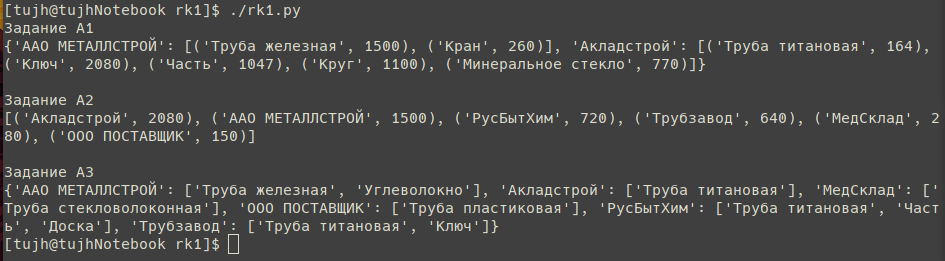
\includegraphics[scale=0.7]{1.png}}
	\end{figure}
	
\end{document}
